%!TEX root = ./report.tex
\section{Problem Analysis and Requirements}
\label{sec:problem_analysis_and_requirements}
In the following section we will analyse the problem, and discuss a set of requirements for a solution that is capable of editing a partial IFC model within a specific domain. This list should be thought of as a guideline for how this problem should ideally be approached.

\subsection{Problem Analysis}
\label{subsec:problem_analysis}
The separation of the construction and plumbing model makes it difficult to work on objects that are interrelated between the two models. We focus on the case of IfcFlowSegments (e.g. a pipe), IfcWallStandardCases (a regular wall) and an IfcOpeningElement (an opening in a regular wall). Jørgensen mentions that a possible solution to the problem is to allow the building service engineer to create a message with precise information about required holes, or openings, for the pipes\,\cite{jorgensen12}. This message could then be handed to the construction engineer, so that he can verify that these are properly placed. As such, the primary goal of the solution is to enable the user to work on a subset of the IFC model involving pipes, openings, and walls. In Figure \ref{fig:ifcheirachy}, a graphical representation of this subset is presented.

\begin{figure}[t]
    \centering
        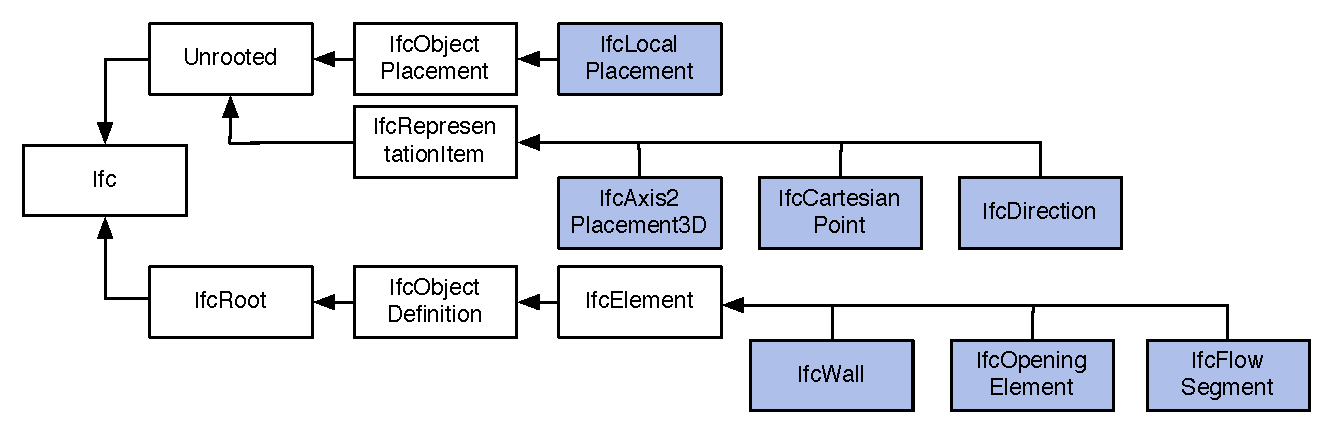
\includegraphics[width=110mm]{images/IfcHeirachy.pdf}
    \caption{A graphical representation of the subset used, excluding relational objects for the sake of simplicity. The objects of the chosen subdomain are highlighted in blue.}
    \label{fig:ifcheirachy}
\end{figure}

\subsection{Requirements}
\label{subsec:requirements}
\subsubsection{Working with a Partial Model}
With the aforementioned complexities and challenges of IFC in mind, a primary focus is to be able to extract a well-specified subset of an IFC model. It is desirable to have an architecture that separates this from the rest of the workflow into one component that extracts the partial model that we are interested in. Reversely, the problem of re-inserting this partial model into the merged IFC model, should also be implemented as an encapsulated workflow component. This should make the components easier to reuse, and make it easier to verify that the transformations are done correctly.

Furthermore, a clear domain definition is needed to implement and verify the extraction of the partial model. Achieving this in a concise but generic way is not trivial. An evolving standard for doing this is via Model View Definitions(MVD)\,\cite{nour08}, which allow fine-grained definitions of IFC subsets using XML. buildingSMART, a non profit organization that supports open source BIM software, propagates MVD as their standard.\footnote{buildingSMART, MVD, \url{http://buildingsmart.com/standards/mvd}} Nour discusses this and other challenges when working with partial editing on IFC\,\cite{nour08}.  Unfortunately, it was not possible to obtain the product of Nour's project. Even though MVD seems to be a promising approach for extracting IFC subsets, it is outside the scope of this project to develop the functionality ourselves. We find that simply defining a partial model with MVD is in itself a somewhat complex task. Therefore, for the purposes of designing a single experimental DSL with only a few IFC classes, we argue that a more informal definition of the domain is sufficient and will simplify the development.

\subsubsection{Correct Meta Model}
It is vital for the solution that the IFC meta model is in fact correct. This point may seem obvious at first, but in our experience, finding a correct EMF meta model that reflects the actual IFC standard is difficult. In particular, finding a model with a proper serializer and deserialiser that converts from either EXPRESS or ifcXML to the corresponding Ecore instance, can be difficult. The difficulty lies in the fact, that across existing BIM software, it is not consistent how IFC models are treated, so one must be aware of inconsistencies\,\cite[p. 4]{quteprints37725}.

\subsubsection{Valid Model Transformations}
An ideal solution would feature model transformations that are verifiable and correct. By verifiable, we mean being able to trace or test that transformations actually occur in the way that we expect. By correct, we primarily mean not corrupting any model structure during a transformation.  However, with the complexity of IFC in mind, we do not require that no constraints are broken in the IFC model at the end of the transformation. As an example, we could imagine that in some IFC models all pipe objects should be referenced from some central entity. It would be difficult to require and assert that no such constraint are broken in the general case, and is a problem outside the scope of this project.

\subsubsection{A Simple DSL}
This being a feasibility study, we only the include a DSL as a proof of concept, so the quality of the syntax or usability of this is less important. One could imagine that a future end product would have a visual syntax instead of a textual syntax.

The simple DSL will demonstrate that the editing of partial model is feasible for our own and similar subdomains of IFC. The implementation will show how a small but significant domain can be managed separately from the IFC model. To support extensibility and reusability, it should be built with widely used tools like the ones of EMF.

\subsubsection{Structural Editing}
It must be possible to use the DSL to add and remove elements. This is required as to resemble a real-world use case scenario, where an element could be missing. The solution must be able to do this, without corrupting the IFC instance.
\paragraph{}
This concludes the list of desirable features, but please note that it is only a core selection and that one could imagine many extensions to it. Some of these will be discussed in Section \ref{sec:plan_for_future_projects} as an idea for a future project.

